% Created by tikzDevice version 0.10.1 on 2018-01-19 13:04:09
% !TEX encoding = UTF-8 Unicode
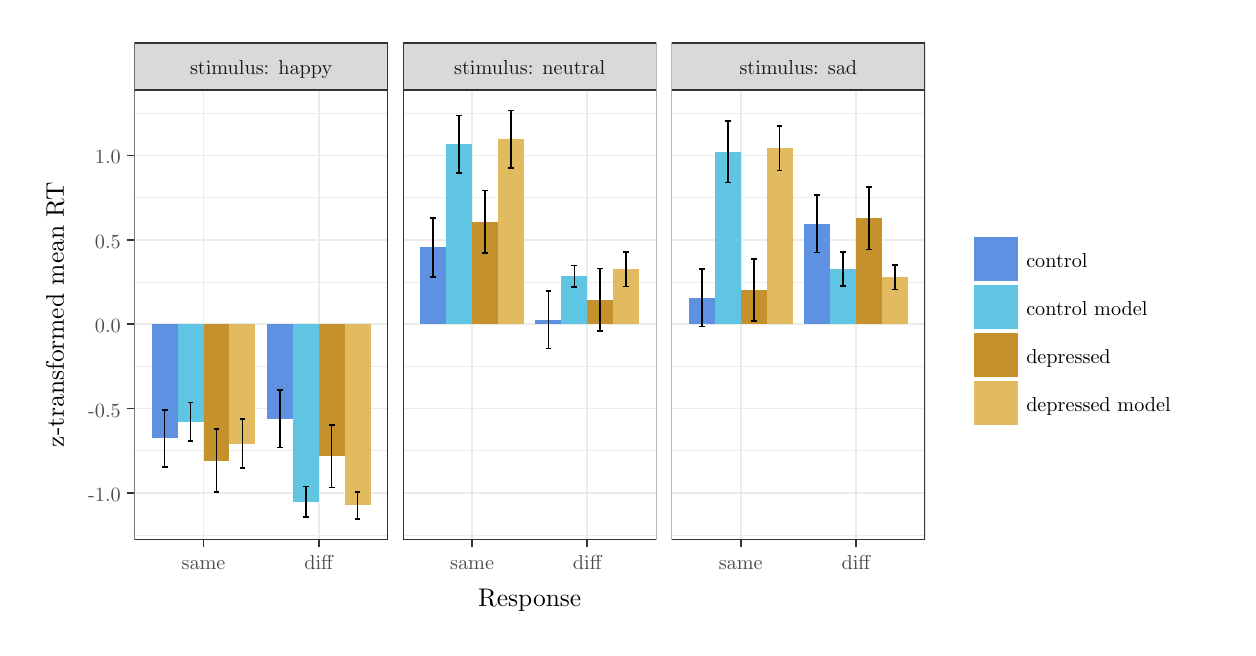
\begin{tikzpicture}[x=1pt,y=1pt]
\definecolor{fillColor}{RGB}{255,255,255}
\path[use as bounding box,fill=fillColor,fill opacity=0.00] (0,0) rectangle (433.62,216.81);
\begin{scope}
\path[clip] (  0.00,  0.00) rectangle (433.62,216.81);
\definecolor{drawColor}{RGB}{255,255,255}
\definecolor{fillColor}{RGB}{255,255,255}

\path[draw=drawColor,line width= 0.6pt,line join=round,line cap=round,fill=fillColor] ( -0.00,  0.00) rectangle (433.62,216.81);
\end{scope}
\begin{scope}
\path[clip] ( 38.57, 31.92) rectangle (130.13,194.25);
\definecolor{fillColor}{RGB}{255,255,255}

\path[fill=fillColor] ( 38.57, 31.92) rectangle (130.13,194.25);
\definecolor{drawColor}{gray}{0.92}

\path[draw=drawColor,line width= 0.3pt,line join=round] ( 38.57, 33.38) --
	(130.13, 33.38);

\path[draw=drawColor,line width= 0.3pt,line join=round] ( 38.57, 63.88) --
	(130.13, 63.88);

\path[draw=drawColor,line width= 0.3pt,line join=round] ( 38.57, 94.39) --
	(130.13, 94.39);

\path[draw=drawColor,line width= 0.3pt,line join=round] ( 38.57,124.89) --
	(130.13,124.89);

\path[draw=drawColor,line width= 0.3pt,line join=round] ( 38.57,155.39) --
	(130.13,155.39);

\path[draw=drawColor,line width= 0.3pt,line join=round] ( 38.57,185.89) --
	(130.13,185.89);

\path[draw=drawColor,line width= 0.6pt,line join=round] ( 38.57, 48.63) --
	(130.13, 48.63);

\path[draw=drawColor,line width= 0.6pt,line join=round] ( 38.57, 79.14) --
	(130.13, 79.14);

\path[draw=drawColor,line width= 0.6pt,line join=round] ( 38.57,109.64) --
	(130.13,109.64);

\path[draw=drawColor,line width= 0.6pt,line join=round] ( 38.57,140.14) --
	(130.13,140.14);

\path[draw=drawColor,line width= 0.6pt,line join=round] ( 38.57,170.64) --
	(130.13,170.64);

\path[draw=drawColor,line width= 0.6pt,line join=round] ( 63.54, 31.92) --
	( 63.54,194.25);

\path[draw=drawColor,line width= 0.6pt,line join=round] (105.16, 31.92) --
	(105.16,194.25);
\definecolor{fillColor}{RGB}{226,186,95}

\path[fill=fillColor] ( 72.91, 66.50) rectangle ( 82.27,109.64);
\definecolor{fillColor}{RGB}{196,145,45}

\path[fill=fillColor] ( 63.54, 60.40) rectangle ( 72.91,109.64);
\definecolor{fillColor}{RGB}{95,197,226}

\path[fill=fillColor] ( 54.18, 74.40) rectangle ( 63.54,109.64);
\definecolor{fillColor}{RGB}{95,145,226}

\path[fill=fillColor] ( 44.81, 68.36) rectangle ( 54.18,109.64);
\definecolor{fillColor}{RGB}{226,186,95}

\path[fill=fillColor] (114.52, 44.19) rectangle (123.89,109.64);
\definecolor{fillColor}{RGB}{196,145,45}

\path[fill=fillColor] (105.16, 61.99) rectangle (114.52,109.64);
\definecolor{fillColor}{RGB}{95,197,226}

\path[fill=fillColor] ( 95.80, 45.58) rectangle (105.16,109.64);
\definecolor{fillColor}{RGB}{95,145,226}

\path[fill=fillColor] ( 86.43, 75.45) rectangle ( 95.80,109.64);
\definecolor{drawColor}{RGB}{0,0,0}

\path[draw=drawColor,line width= 0.6pt,line join=round] ( 76.55, 75.32) --
	( 78.63, 75.32);

\path[draw=drawColor,line width= 0.6pt,line join=round] ( 77.59, 75.32) --
	( 77.59, 57.67);

\path[draw=drawColor,line width= 0.6pt,line join=round] ( 76.55, 57.67) --
	( 78.63, 57.67);

\path[draw=drawColor,line width= 0.6pt,line join=round] ( 67.18, 71.68) --
	( 69.26, 71.68);

\path[draw=drawColor,line width= 0.6pt,line join=round] ( 68.22, 71.68) --
	( 68.22, 49.12);

\path[draw=drawColor,line width= 0.6pt,line join=round] ( 67.18, 49.12) --
	( 69.26, 49.12);

\path[draw=drawColor,line width= 0.6pt,line join=round] ( 57.82, 81.34) --
	( 59.90, 81.34);

\path[draw=drawColor,line width= 0.6pt,line join=round] ( 58.86, 81.34) --
	( 58.86, 67.45);

\path[draw=drawColor,line width= 0.6pt,line join=round] ( 57.82, 67.45) --
	( 59.90, 67.45);

\path[draw=drawColor,line width= 0.6pt,line join=round] ( 48.46, 78.73) --
	( 50.54, 78.73);

\path[draw=drawColor,line width= 0.6pt,line join=round] ( 49.50, 78.73) --
	( 49.50, 57.99);

\path[draw=drawColor,line width= 0.6pt,line join=round] ( 48.46, 57.99) --
	( 50.54, 57.99);

\path[draw=drawColor,line width= 0.6pt,line join=round] (118.17, 49.09) --
	(120.25, 49.09);

\path[draw=drawColor,line width= 0.6pt,line join=round] (119.21, 49.09) --
	(119.21, 39.30);

\path[draw=drawColor,line width= 0.6pt,line join=round] (118.17, 39.30) --
	(120.25, 39.30);

\path[draw=drawColor,line width= 0.6pt,line join=round] (108.80, 73.28) --
	(110.88, 73.28);

\path[draw=drawColor,line width= 0.6pt,line join=round] (109.84, 73.28) --
	(109.84, 50.71);

\path[draw=drawColor,line width= 0.6pt,line join=round] (108.80, 50.71) --
	(110.88, 50.71);

\path[draw=drawColor,line width= 0.6pt,line join=round] ( 99.44, 51.07) --
	(101.52, 51.07);

\path[draw=drawColor,line width= 0.6pt,line join=round] (100.48, 51.07) --
	(100.48, 40.08);

\path[draw=drawColor,line width= 0.6pt,line join=round] ( 99.44, 40.08) --
	(101.52, 40.08);

\path[draw=drawColor,line width= 0.6pt,line join=round] ( 90.07, 85.84) --
	( 92.15, 85.84);

\path[draw=drawColor,line width= 0.6pt,line join=round] ( 91.11, 85.84) --
	( 91.11, 65.05);

\path[draw=drawColor,line width= 0.6pt,line join=round] ( 90.07, 65.05) --
	( 92.15, 65.05);
\definecolor{drawColor}{gray}{0.20}

\path[draw=drawColor,line width= 0.6pt,line join=round,line cap=round] ( 38.57, 31.92) rectangle (130.13,194.25);
\end{scope}
\begin{scope}
\path[clip] (135.63, 31.92) rectangle (227.19,194.25);
\definecolor{fillColor}{RGB}{255,255,255}

\path[fill=fillColor] (135.63, 31.92) rectangle (227.19,194.25);
\definecolor{drawColor}{gray}{0.92}

\path[draw=drawColor,line width= 0.3pt,line join=round] (135.63, 33.38) --
	(227.19, 33.38);

\path[draw=drawColor,line width= 0.3pt,line join=round] (135.63, 63.88) --
	(227.19, 63.88);

\path[draw=drawColor,line width= 0.3pt,line join=round] (135.63, 94.39) --
	(227.19, 94.39);

\path[draw=drawColor,line width= 0.3pt,line join=round] (135.63,124.89) --
	(227.19,124.89);

\path[draw=drawColor,line width= 0.3pt,line join=round] (135.63,155.39) --
	(227.19,155.39);

\path[draw=drawColor,line width= 0.3pt,line join=round] (135.63,185.89) --
	(227.19,185.89);

\path[draw=drawColor,line width= 0.6pt,line join=round] (135.63, 48.63) --
	(227.19, 48.63);

\path[draw=drawColor,line width= 0.6pt,line join=round] (135.63, 79.14) --
	(227.19, 79.14);

\path[draw=drawColor,line width= 0.6pt,line join=round] (135.63,109.64) --
	(227.19,109.64);

\path[draw=drawColor,line width= 0.6pt,line join=round] (135.63,140.14) --
	(227.19,140.14);

\path[draw=drawColor,line width= 0.6pt,line join=round] (135.63,170.64) --
	(227.19,170.64);

\path[draw=drawColor,line width= 0.6pt,line join=round] (160.60, 31.92) --
	(160.60,194.25);

\path[draw=drawColor,line width= 0.6pt,line join=round] (202.22, 31.92) --
	(202.22,194.25);
\definecolor{fillColor}{RGB}{226,186,95}

\path[fill=fillColor] (169.97,109.64) rectangle (179.33,176.53);
\definecolor{fillColor}{RGB}{196,145,45}

\path[fill=fillColor] (160.60,109.64) rectangle (169.97,146.63);
\definecolor{fillColor}{RGB}{95,197,226}

\path[fill=fillColor] (151.24,109.64) rectangle (160.60,174.69);
\definecolor{fillColor}{RGB}{95,145,226}

\path[fill=fillColor] (141.87,109.64) rectangle (151.24,137.47);
\definecolor{fillColor}{RGB}{226,186,95}

\path[fill=fillColor] (211.59,109.64) rectangle (220.95,129.54);
\definecolor{fillColor}{RGB}{196,145,45}

\path[fill=fillColor] (202.22,109.64) rectangle (211.59,118.42);
\definecolor{fillColor}{RGB}{95,197,226}

\path[fill=fillColor] (192.86,109.64) rectangle (202.22,127.05);
\definecolor{fillColor}{RGB}{95,145,226}

\path[fill=fillColor] (183.49,109.64) rectangle (192.86,111.23);
\definecolor{drawColor}{RGB}{0,0,0}

\path[draw=drawColor,line width= 0.6pt,line join=round] (173.61,186.87) --
	(175.69,186.87);

\path[draw=drawColor,line width= 0.6pt,line join=round] (174.65,186.87) --
	(174.65,166.19);

\path[draw=drawColor,line width= 0.6pt,line join=round] (173.61,166.19) --
	(175.69,166.19);

\path[draw=drawColor,line width= 0.6pt,line join=round] (164.24,157.91) --
	(166.33,157.91);

\path[draw=drawColor,line width= 0.6pt,line join=round] (165.28,157.91) --
	(165.28,135.34);

\path[draw=drawColor,line width= 0.6pt,line join=round] (164.24,135.34) --
	(166.33,135.34);

\path[draw=drawColor,line width= 0.6pt,line join=round] (154.88,185.01) --
	(156.96,185.01);

\path[draw=drawColor,line width= 0.6pt,line join=round] (155.92,185.01) --
	(155.92,164.38);

\path[draw=drawColor,line width= 0.6pt,line join=round] (154.88,164.38) --
	(156.96,164.38);

\path[draw=drawColor,line width= 0.6pt,line join=round] (145.52,148.10) --
	(147.60,148.10);

\path[draw=drawColor,line width= 0.6pt,line join=round] (146.56,148.10) --
	(146.56,126.83);

\path[draw=drawColor,line width= 0.6pt,line join=round] (145.52,126.83) --
	(147.60,126.83);

\path[draw=drawColor,line width= 0.6pt,line join=round] (215.23,135.78) --
	(217.31,135.78);

\path[draw=drawColor,line width= 0.6pt,line join=round] (216.27,135.78) --
	(216.27,123.31);

\path[draw=drawColor,line width= 0.6pt,line join=round] (215.23,123.31) --
	(217.31,123.31);

\path[draw=drawColor,line width= 0.6pt,line join=round] (205.86,129.73) --
	(207.94,129.73);

\path[draw=drawColor,line width= 0.6pt,line join=round] (206.90,129.73) --
	(206.90,107.11);

\path[draw=drawColor,line width= 0.6pt,line join=round] (205.86,107.11) --
	(207.94,107.11);

\path[draw=drawColor,line width= 0.6pt,line join=round] (196.50,130.92) --
	(198.58,130.92);

\path[draw=drawColor,line width= 0.6pt,line join=round] (197.54,130.92) --
	(197.54,123.18);

\path[draw=drawColor,line width= 0.6pt,line join=round] (196.50,123.18) --
	(198.58,123.18);

\path[draw=drawColor,line width= 0.6pt,line join=round] (187.13,121.60) --
	(189.22,121.60);

\path[draw=drawColor,line width= 0.6pt,line join=round] (188.18,121.60) --
	(188.18,100.86);

\path[draw=drawColor,line width= 0.6pt,line join=round] (187.13,100.86) --
	(189.22,100.86);
\definecolor{drawColor}{gray}{0.20}

\path[draw=drawColor,line width= 0.6pt,line join=round,line cap=round] (135.63, 31.92) rectangle (227.19,194.25);
\end{scope}
\begin{scope}
\path[clip] (232.69, 31.92) rectangle (324.25,194.25);
\definecolor{fillColor}{RGB}{255,255,255}

\path[fill=fillColor] (232.69, 31.92) rectangle (324.25,194.25);
\definecolor{drawColor}{gray}{0.92}

\path[draw=drawColor,line width= 0.3pt,line join=round] (232.69, 33.38) --
	(324.25, 33.38);

\path[draw=drawColor,line width= 0.3pt,line join=round] (232.69, 63.88) --
	(324.25, 63.88);

\path[draw=drawColor,line width= 0.3pt,line join=round] (232.69, 94.39) --
	(324.25, 94.39);

\path[draw=drawColor,line width= 0.3pt,line join=round] (232.69,124.89) --
	(324.25,124.89);

\path[draw=drawColor,line width= 0.3pt,line join=round] (232.69,155.39) --
	(324.25,155.39);

\path[draw=drawColor,line width= 0.3pt,line join=round] (232.69,185.89) --
	(324.25,185.89);

\path[draw=drawColor,line width= 0.6pt,line join=round] (232.69, 48.63) --
	(324.25, 48.63);

\path[draw=drawColor,line width= 0.6pt,line join=round] (232.69, 79.14) --
	(324.25, 79.14);

\path[draw=drawColor,line width= 0.6pt,line join=round] (232.69,109.64) --
	(324.25,109.64);

\path[draw=drawColor,line width= 0.6pt,line join=round] (232.69,140.14) --
	(324.25,140.14);

\path[draw=drawColor,line width= 0.6pt,line join=round] (232.69,170.64) --
	(324.25,170.64);

\path[draw=drawColor,line width= 0.6pt,line join=round] (257.66, 31.92) --
	(257.66,194.25);

\path[draw=drawColor,line width= 0.6pt,line join=round] (299.28, 31.92) --
	(299.28,194.25);
\definecolor{fillColor}{RGB}{226,186,95}

\path[fill=fillColor] (267.03,109.64) rectangle (276.39,173.28);
\definecolor{fillColor}{RGB}{196,145,45}

\path[fill=fillColor] (257.66,109.64) rectangle (267.03,121.98);
\definecolor{fillColor}{RGB}{95,197,226}

\path[fill=fillColor] (248.30,109.64) rectangle (257.66,171.98);
\definecolor{fillColor}{RGB}{95,145,226}

\path[fill=fillColor] (238.94,109.64) rectangle (248.30,119.14);
\definecolor{fillColor}{RGB}{226,186,95}

\path[fill=fillColor] (308.65,109.64) rectangle (318.01,126.59);
\definecolor{fillColor}{RGB}{196,145,45}

\path[fill=fillColor] (299.28,109.64) rectangle (308.65,147.98);
\definecolor{fillColor}{RGB}{95,197,226}

\path[fill=fillColor] (289.92,109.64) rectangle (299.28,129.62);
\definecolor{fillColor}{RGB}{95,145,226}

\path[fill=fillColor] (280.55,109.64) rectangle (289.92,145.91);
\definecolor{drawColor}{RGB}{0,0,0}

\path[draw=drawColor,line width= 0.6pt,line join=round] (270.67,181.37) --
	(272.75,181.37);

\path[draw=drawColor,line width= 0.6pt,line join=round] (271.71,181.37) --
	(271.71,165.20);

\path[draw=drawColor,line width= 0.6pt,line join=round] (270.67,165.20) --
	(272.75,165.20);

\path[draw=drawColor,line width= 0.6pt,line join=round] (261.31,133.27) --
	(263.39,133.27);

\path[draw=drawColor,line width= 0.6pt,line join=round] (262.35,133.27) --
	(262.35,110.70);

\path[draw=drawColor,line width= 0.6pt,line join=round] (261.31,110.70) --
	(263.39,110.70);

\path[draw=drawColor,line width= 0.6pt,line join=round] (251.94,183.10) --
	(254.02,183.10);

\path[draw=drawColor,line width= 0.6pt,line join=round] (252.98,183.10) --
	(252.98,160.86);

\path[draw=drawColor,line width= 0.6pt,line join=round] (251.94,160.86) --
	(254.02,160.86);

\path[draw=drawColor,line width= 0.6pt,line join=round] (242.58,129.51) --
	(244.66,129.51);

\path[draw=drawColor,line width= 0.6pt,line join=round] (243.62,129.51) --
	(243.62,108.77);

\path[draw=drawColor,line width= 0.6pt,line join=round] (242.58,108.77) --
	(244.66,108.77);

\path[draw=drawColor,line width= 0.6pt,line join=round] (312.29,130.97) --
	(314.37,130.97);

\path[draw=drawColor,line width= 0.6pt,line join=round] (313.33,130.97) --
	(313.33,122.21);

\path[draw=drawColor,line width= 0.6pt,line join=round] (312.29,122.21) --
	(314.37,122.21);

\path[draw=drawColor,line width= 0.6pt,line join=round] (302.92,159.29) --
	(305.00,159.29);

\path[draw=drawColor,line width= 0.6pt,line join=round] (303.96,159.29) --
	(303.96,136.67);

\path[draw=drawColor,line width= 0.6pt,line join=round] (302.92,136.67) --
	(305.00,136.67);

\path[draw=drawColor,line width= 0.6pt,line join=round] (293.56,135.80) --
	(295.64,135.80);

\path[draw=drawColor,line width= 0.6pt,line join=round] (294.60,135.80) --
	(294.60,123.45);

\path[draw=drawColor,line width= 0.6pt,line join=round] (293.56,123.45) --
	(295.64,123.45);

\path[draw=drawColor,line width= 0.6pt,line join=round] (284.20,156.27) --
	(286.28,156.27);

\path[draw=drawColor,line width= 0.6pt,line join=round] (285.24,156.27) --
	(285.24,135.54);

\path[draw=drawColor,line width= 0.6pt,line join=round] (284.20,135.54) --
	(286.28,135.54);
\definecolor{drawColor}{gray}{0.20}

\path[draw=drawColor,line width= 0.6pt,line join=round,line cap=round] (232.69, 31.92) rectangle (324.25,194.25);
\end{scope}
\begin{scope}
\path[clip] ( 38.57,194.25) rectangle (130.13,211.31);
\definecolor{drawColor}{gray}{0.20}
\definecolor{fillColor}{gray}{0.85}

\path[draw=drawColor,line width= 0.6pt,line join=round,line cap=round,fill=fillColor] ( 38.57,194.25) rectangle (130.13,211.31);
\definecolor{drawColor}{gray}{0.10}

\node[text=drawColor,anchor=base,inner sep=0pt, outer sep=0pt, scale=  0.73] at ( 84.35,199.75) {stimulus: happy};
\end{scope}
\begin{scope}
\path[clip] (135.63,194.25) rectangle (227.19,211.31);
\definecolor{drawColor}{gray}{0.20}
\definecolor{fillColor}{gray}{0.85}

\path[draw=drawColor,line width= 0.6pt,line join=round,line cap=round,fill=fillColor] (135.63,194.25) rectangle (227.19,211.31);
\definecolor{drawColor}{gray}{0.10}

\node[text=drawColor,anchor=base,inner sep=0pt, outer sep=0pt, scale=  0.73] at (181.41,199.75) {stimulus: neutral};
\end{scope}
\begin{scope}
\path[clip] (232.69,194.25) rectangle (324.25,211.31);
\definecolor{drawColor}{gray}{0.20}
\definecolor{fillColor}{gray}{0.85}

\path[draw=drawColor,line width= 0.6pt,line join=round,line cap=round,fill=fillColor] (232.69,194.25) rectangle (324.25,211.31);
\definecolor{drawColor}{gray}{0.10}

\node[text=drawColor,anchor=base,inner sep=0pt, outer sep=0pt, scale=  0.73] at (278.47,199.75) {stimulus: sad};
\end{scope}
\begin{scope}
\path[clip] (  0.00,  0.00) rectangle (433.62,216.81);
\definecolor{drawColor}{gray}{0.20}

\path[draw=drawColor,line width= 0.6pt,line join=round] ( 63.54, 29.17) --
	( 63.54, 31.92);

\path[draw=drawColor,line width= 0.6pt,line join=round] (105.16, 29.17) --
	(105.16, 31.92);
\end{scope}
\begin{scope}
\path[clip] (  0.00,  0.00) rectangle (433.62,216.81);
\definecolor{drawColor}{gray}{0.30}

\node[text=drawColor,anchor=base,inner sep=0pt, outer sep=0pt, scale=  0.73] at ( 63.54, 20.91) {same};

\node[text=drawColor,anchor=base,inner sep=0pt, outer sep=0pt, scale=  0.73] at (105.16, 20.91) {diff};
\end{scope}
\begin{scope}
\path[clip] (  0.00,  0.00) rectangle (433.62,216.81);
\definecolor{drawColor}{gray}{0.20}

\path[draw=drawColor,line width= 0.6pt,line join=round] (160.60, 29.17) --
	(160.60, 31.92);

\path[draw=drawColor,line width= 0.6pt,line join=round] (202.22, 29.17) --
	(202.22, 31.92);
\end{scope}
\begin{scope}
\path[clip] (  0.00,  0.00) rectangle (433.62,216.81);
\definecolor{drawColor}{gray}{0.30}

\node[text=drawColor,anchor=base,inner sep=0pt, outer sep=0pt, scale=  0.73] at (160.60, 20.91) {same};

\node[text=drawColor,anchor=base,inner sep=0pt, outer sep=0pt, scale=  0.73] at (202.22, 20.91) {diff};
\end{scope}
\begin{scope}
\path[clip] (  0.00,  0.00) rectangle (433.62,216.81);
\definecolor{drawColor}{gray}{0.20}

\path[draw=drawColor,line width= 0.6pt,line join=round] (257.66, 29.17) --
	(257.66, 31.92);

\path[draw=drawColor,line width= 0.6pt,line join=round] (299.28, 29.17) --
	(299.28, 31.92);
\end{scope}
\begin{scope}
\path[clip] (  0.00,  0.00) rectangle (433.62,216.81);
\definecolor{drawColor}{gray}{0.30}

\node[text=drawColor,anchor=base,inner sep=0pt, outer sep=0pt, scale=  0.73] at (257.66, 20.91) {same};

\node[text=drawColor,anchor=base,inner sep=0pt, outer sep=0pt, scale=  0.73] at (299.28, 20.91) {diff};
\end{scope}
\begin{scope}
\path[clip] (  0.00,  0.00) rectangle (433.62,216.81);
\definecolor{drawColor}{gray}{0.30}

\node[text=drawColor,anchor=base east,inner sep=0pt, outer sep=0pt, scale=  0.73] at ( 33.62, 45.60) {-1.0};

\node[text=drawColor,anchor=base east,inner sep=0pt, outer sep=0pt, scale=  0.73] at ( 33.62, 76.11) {-0.5};

\node[text=drawColor,anchor=base east,inner sep=0pt, outer sep=0pt, scale=  0.73] at ( 33.62,106.61) {0.0};

\node[text=drawColor,anchor=base east,inner sep=0pt, outer sep=0pt, scale=  0.73] at ( 33.62,137.11) {0.5};

\node[text=drawColor,anchor=base east,inner sep=0pt, outer sep=0pt, scale=  0.73] at ( 33.62,167.61) {1.0};
\end{scope}
\begin{scope}
\path[clip] (  0.00,  0.00) rectangle (433.62,216.81);
\definecolor{drawColor}{gray}{0.20}

\path[draw=drawColor,line width= 0.6pt,line join=round] ( 35.82, 48.63) --
	( 38.57, 48.63);

\path[draw=drawColor,line width= 0.6pt,line join=round] ( 35.82, 79.14) --
	( 38.57, 79.14);

\path[draw=drawColor,line width= 0.6pt,line join=round] ( 35.82,109.64) --
	( 38.57,109.64);

\path[draw=drawColor,line width= 0.6pt,line join=round] ( 35.82,140.14) --
	( 38.57,140.14);

\path[draw=drawColor,line width= 0.6pt,line join=round] ( 35.82,170.64) --
	( 38.57,170.64);
\end{scope}
\begin{scope}
\path[clip] (  0.00,  0.00) rectangle (433.62,216.81);
\definecolor{drawColor}{RGB}{0,0,0}

\node[text=drawColor,anchor=base,inner sep=0pt, outer sep=0pt, scale=  0.92] at (181.41,  7.83) {Response};
\end{scope}
\begin{scope}
\path[clip] (  0.00,  0.00) rectangle (433.62,216.81);
\definecolor{drawColor}{RGB}{0,0,0}

\node[text=drawColor,rotate= 90.00,anchor=base,inner sep=0pt, outer sep=0pt, scale=  0.92] at ( 13.08,113.08) {z-transformed mean RT};
\end{scope}
\begin{scope}
\path[clip] (  0.00,  0.00) rectangle (433.62,216.81);
\definecolor{fillColor}{RGB}{255,255,255}

\path[fill=fillColor] (335.63, 66.75) rectangle (428.12,159.42);
\end{scope}
\begin{scope}
\path[clip] (  0.00,  0.00) rectangle (433.62,216.81);
\definecolor{fillColor}{RGB}{255,255,255}

\path[fill=fillColor] (341.32,124.47) rectangle (358.67,141.82);
\end{scope}
\begin{scope}
\path[clip] (  0.00,  0.00) rectangle (433.62,216.81);
\definecolor{fillColor}{RGB}{95,145,226}

\path[fill=fillColor] (342.04,125.18) rectangle (357.96,141.11);
\end{scope}
\begin{scope}
\path[clip] (  0.00,  0.00) rectangle (433.62,216.81);
\definecolor{fillColor}{RGB}{255,255,255}

\path[fill=fillColor] (341.32,107.13) rectangle (358.67,124.47);
\end{scope}
\begin{scope}
\path[clip] (  0.00,  0.00) rectangle (433.62,216.81);
\definecolor{fillColor}{RGB}{95,197,226}

\path[fill=fillColor] (342.04,107.84) rectangle (357.96,123.76);
\end{scope}
\begin{scope}
\path[clip] (  0.00,  0.00) rectangle (433.62,216.81);
\definecolor{fillColor}{RGB}{255,255,255}

\path[fill=fillColor] (341.32, 89.78) rectangle (358.67,107.13);
\end{scope}
\begin{scope}
\path[clip] (  0.00,  0.00) rectangle (433.62,216.81);
\definecolor{fillColor}{RGB}{196,145,45}

\path[fill=fillColor] (342.04, 90.49) rectangle (357.96,106.42);
\end{scope}
\begin{scope}
\path[clip] (  0.00,  0.00) rectangle (433.62,216.81);
\definecolor{fillColor}{RGB}{255,255,255}

\path[fill=fillColor] (341.32, 72.44) rectangle (358.67, 89.78);
\end{scope}
\begin{scope}
\path[clip] (  0.00,  0.00) rectangle (433.62,216.81);
\definecolor{fillColor}{RGB}{226,186,95}

\path[fill=fillColor] (342.04, 73.15) rectangle (357.96, 89.07);
\end{scope}
\begin{scope}
\path[clip] (  0.00,  0.00) rectangle (433.62,216.81);
\definecolor{drawColor}{RGB}{0,0,0}

\node[text=drawColor,anchor=base west,inner sep=0pt, outer sep=0pt, scale=  0.73] at (360.84,130.12) {control};
\end{scope}
\begin{scope}
\path[clip] (  0.00,  0.00) rectangle (433.62,216.81);
\definecolor{drawColor}{RGB}{0,0,0}

\node[text=drawColor,anchor=base west,inner sep=0pt, outer sep=0pt, scale=  0.73] at (360.84,112.77) {control model};
\end{scope}
\begin{scope}
\path[clip] (  0.00,  0.00) rectangle (433.62,216.81);
\definecolor{drawColor}{RGB}{0,0,0}

\node[text=drawColor,anchor=base west,inner sep=0pt, outer sep=0pt, scale=  0.73] at (360.84, 95.43) {depressed};
\end{scope}
\begin{scope}
\path[clip] (  0.00,  0.00) rectangle (433.62,216.81);
\definecolor{drawColor}{RGB}{0,0,0}

\node[text=drawColor,anchor=base west,inner sep=0pt, outer sep=0pt, scale=  0.73] at (360.84, 78.08) {depressed model};
\end{scope}
\end{tikzpicture}
